% ============================================================
%  OOPS and DSA in Python — Comprehensive Reference Document
%  Covers: OOP, Data Structures, Algorithms, Modern Structures,
%          Data Management and Governance
%  Diagrams: TikZ (trees, graphs, linked lists, hash tables, etc.)
%  References: CLRS, Sedgewick, Knuth, Goodrich et al.
% ============================================================
\documentclass[12pt,a4paper]{article}

% ---------- packages ----------
\usepackage[T1]{fontenc}
\usepackage[utf8]{inputenc}
\usepackage{lmodern}
\usepackage[margin=2.5cm]{geometry}
\usepackage{amsmath,amssymb,amsthm}
\usepackage{algorithm}
\usepackage[noend]{algpseudocode}
\usepackage{listings}
\usepackage{xcolor}
\usepackage{tikz}
\usepackage{tikz-qtree}
\usepackage{forest}
\usepackage{pgfplots}
\pgfplotsset{compat=1.18}
\usepackage{hyperref}
\usepackage{booktabs}
\usepackage{multirow}
\usepackage{enumitem}
\usepackage{caption}
\usepackage{subcaption}
\usepackage[backend=biber,style=authoryear,sorting=nyt]{biblatex}

\usetikzlibrary{
  shapes.geometric,
  shapes.multipart,
  arrows.meta,
  arrows,
  positioning,
  fit,
  backgrounds,
  decorations.pathreplacing,
  calc,
  matrix,
  chains,
  scopes
}

% ---------- colours ----------
\definecolor{pyblue}{RGB}{30,100,200}
\definecolor{pygray}{RGB}{60,60,60}
\definecolor{pygreen}{RGB}{0,128,0}
\definecolor{pyred}{RGB}{180,0,0}
\definecolor{pylightblue}{RGB}{220,235,255}
\definecolor{pylightgreen}{RGB}{220,255,220}
\definecolor{nodegray}{RGB}{220,220,220}
\definecolor{nodeorange}{RGB}{255,200,100}
\definecolor{nodeblue}{RGB}{100,180,255}
\definecolor{nodered}{RGB}{255,120,120}

% ---------- listings style ----------
\lstdefinestyle{python}{
  language=Python,
  basicstyle=\ttfamily\small,
  keywordstyle=\color{pyblue}\bfseries,
  commentstyle=\color{pygreen}\itshape,
  stringstyle=\color{pyred},
  numberstyle=\tiny\color{pygray},
  numbers=left,
  stepnumber=1,
  tabsize=4,
  showstringspaces=false,
  breaklines=true,
  frame=single,
  rulecolor=\color{pygray!40},
  backgroundcolor=\color{pylightblue!30},
  captionpos=b
}
\lstset{style=python}

% ---------- theorem environments ----------
\newtheorem{theorem}{Theorem}[section]
\newtheorem{lemma}[theorem]{Lemma}
\newtheorem{definition}{Definition}[section]
\newtheorem{complexity}{Complexity}[section]

% ---------- bibliography ----------
\addbibresource{references.bib}

% ---------- metadata ----------
\title{%
  \textbf{Object-Oriented Programming and Data Structures \& Algorithms in Python}\\
  \large From Foundational Concepts to Modern Data Management and Governance
}
\author{Reference Guide with TikZ Diagrams and Academic Citations}
\date{\today}

% ============================================================
\begin{document}
\maketitle
\tableofcontents
\clearpage

% ============================================================
\section{Introduction}
% ============================================================

This document provides a comprehensive, academically referenced guide to
\textbf{Object-Oriented Programming (OOP)}, classical and modern
\textbf{Data Structures}, and \textbf{Algorithm Design} in the Python
programming language.  All code examples target Python~3.11+.

The treatment follows the curriculum of seminal textbooks
\cite{cormen2022,sedgewick2011,knuth1997v1,goodrich2013},
and is enriched with findings from landmark research papers
\cite{bloom1970,pugh1990,dijkstra1959,kruskal1956,tarjan1975}.

% ============================================================
\section{Object-Oriented Programming}
% ============================================================

\subsection{Core Pillars}

\begin{definition}[Class]
A \emph{class} is a user-defined data type that encapsulates data (attributes)
and behaviour (methods) into a single logical unit~\cite{goodrich2013}.
\end{definition}

The four foundational pillars of OOP are illustrated in
Figure~\ref{fig:oop-pillars}.

\begin{figure}[h]
\centering
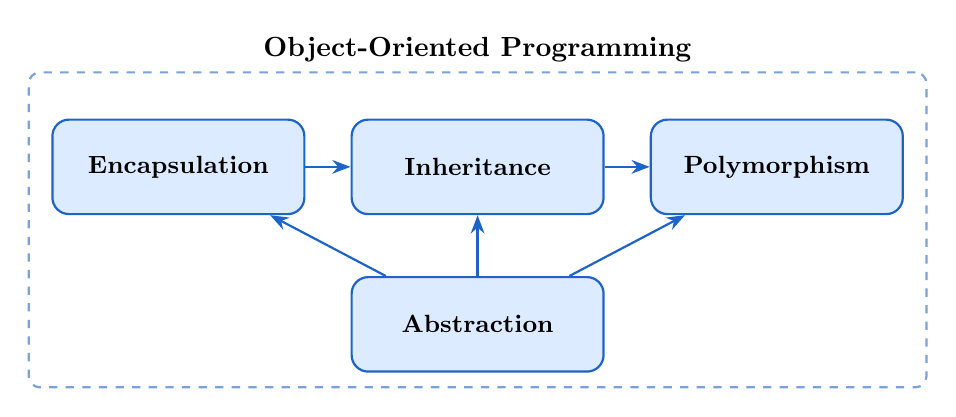
\begin{tikzpicture}[
  pillar/.style={
    rectangle, rounded corners=6pt,
    minimum width=3.2cm, minimum height=1.2cm,
    draw=pyblue, fill=pylightblue, thick,
    font=\bfseries\small
  },
  arrow/.style={-Stealth, thick, pyblue}
]
  \node[pillar] (enc) at (0,0)     {Encapsulation};
  \node[pillar] (inh) at (3.8,0)   {Inheritance};
  \node[pillar] (pol) at (7.6,0)   {Polymorphism};
  \node[pillar] (abs) at (3.8,-2)  {Abstraction};

  \node[rectangle, rounded corners=4pt,
        minimum width=11.4cm, minimum height=4cm,
        draw=pyblue!60, dashed, thick, label=above:\textbf{Object-Oriented Programming}]
       at (3.8,-0.8) {};

  \draw[arrow] (enc) -- (inh);
  \draw[arrow] (inh) -- (pol);
  \draw[arrow] (abs) -- (enc);
  \draw[arrow] (abs) -- (inh);
  \draw[arrow] (abs) -- (pol);
\end{tikzpicture}
\caption{The four pillars of Object-Oriented Programming and their relationships.}
\label{fig:oop-pillars}
\end{figure}

\subsection{Inheritance Hierarchy}

Figure~\ref{fig:inheritance} shows a sample class hierarchy for geometric shapes.

\begin{figure}[h]
\centering
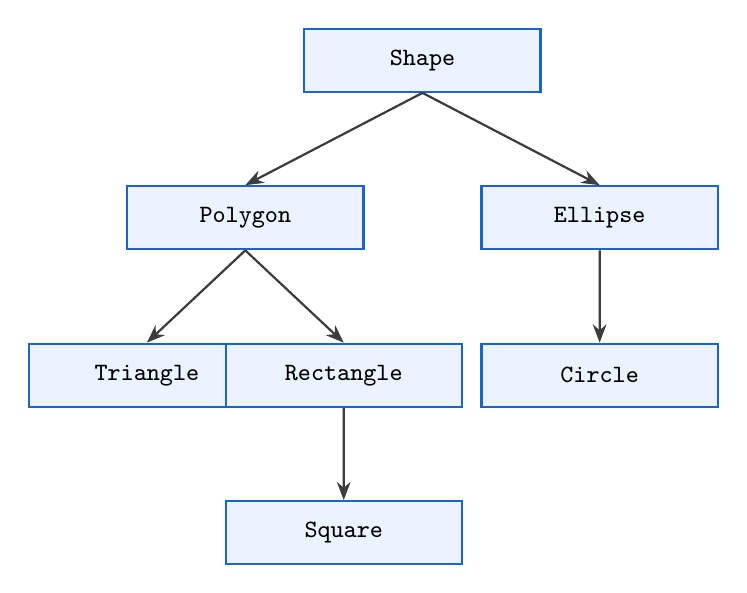
\begin{tikzpicture}[
  class/.style={
    rectangle, draw=pyblue, fill=pylightblue!60, thick,
    minimum width=3cm, minimum height=0.8cm, font=\ttfamily\small
  },
  edge from parent/.style={draw=pygray, -Stealth, thick},
  level 1/.style={sibling distance=4.5cm, level distance=2cm},
  level 2/.style={sibling distance=2.5cm, level distance=2cm}
]
  \node[class] {Shape}
    child { node[class] {Polygon}
      child { node[class] {Triangle} }
      child { node[class] {Rectangle}
        child { node[class] {Square} }
      }
    }
    child { node[class] {Ellipse}
      child { node[class] {Circle} }
    };
\end{tikzpicture}
\caption{Inheritance hierarchy for geometric shapes in Python.}
\label{fig:inheritance}
\end{figure}

\subsection{Design Patterns}

\begin{table}[h]
\centering
\caption{Gang-of-Four design patterns commonly used in Python~\cite{gamma1994}.}
\begin{tabular}{llp{6cm}}
\toprule
\textbf{Category} & \textbf{Pattern} & \textbf{Intent} \\
\midrule
Creational & Singleton & Ensure a class has only one instance \\
           & Factory Method & Defer object creation to subclasses \\
           & Builder & Construct complex objects step by step \\
\midrule
Structural & Decorator & Attach additional responsibilities dynamically \\
           & Adapter   & Convert an interface into another \\
           & Composite & Treat individual objects and compositions uniformly \\
\midrule
Behavioural & Observer  & Notify dependants of state changes \\
            & Strategy  & Encapsulate interchangeable algorithms \\
            & Iterator  & Provide sequential access to elements \\
\bottomrule
\end{tabular}
\end{table}

% ============================================================
\section{Linear Data Structures}
% ============================================================

\subsection{Arrays and Lists}

Python's built-in \texttt{list} is a \emph{dynamic array}:
it maintains a contiguous block of pointers and doubles its allocated
capacity on overflow, giving amortised $O(1)$ append~\cite{goodrich2013}.

\begin{complexity}[Dynamic Array Operations]
\label{cplx:array}
Let $n$ be the number of elements.
\[
  \text{Access}: O(1) \quad
  \text{Append}^*: O(1) \quad
  \text{Insert at } i: O(n) \quad
  \text{Delete at } i: O(n)
\]
where $^*$ denotes amortised complexity.
\end{complexity}

\subsection{Linked Lists}

Figure~\ref{fig:linked-list} illustrates a singly linked list with four nodes.

\begin{figure}[h]
\centering
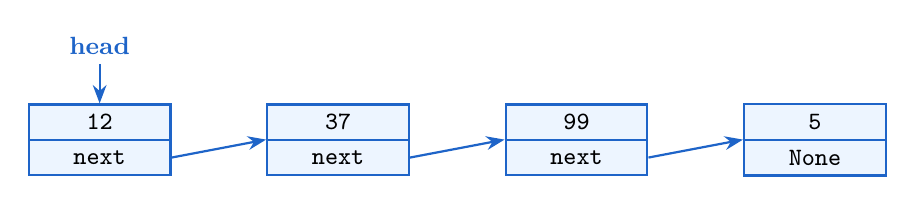
\begin{tikzpicture}[
  node distance=0.4cm,
  box/.style={
    rectangle split, rectangle split parts=2,
    draw=pyblue, fill=pylightblue!50, thick,
    minimum width=1.8cm, minimum height=0.9cm,
    font=\ttfamily\small
  },
  ptr/.style={-Stealth, thick, pyblue}
]
  \node[box] (n1) {\textbf{12} \nodepart{second} next};
  \node[box, right=1.2cm of n1] (n2) {\textbf{37} \nodepart{second} next};
  \node[box, right=1.2cm of n2] (n3) {\textbf{99} \nodepart{second} next};
  \node[box, right=1.2cm of n3] (n4) {\textbf{5}  \nodepart{second} None};

  \draw[ptr] (n1.two east) -- (n2.west);
  \draw[ptr] (n2.two east) -- (n3.west);
  \draw[ptr] (n3.two east) -- (n4.west);

  \node[above=0.5cm of n1, font=\bfseries\small, pyblue] (head) {head};
  \draw[ptr] (head) -- (n1.north);
\end{tikzpicture}
\caption{Singly linked list: \texttt{head} $\to$ 12 $\to$ 37 $\to$ 99 $\to$ 5 $\to$ \texttt{None}.}
\label{fig:linked-list}
\end{figure}

\subsection{Stacks and Queues}

\begin{figure}[h]
\centering
\begin{subfigure}[b]{0.45\textwidth}
\centering
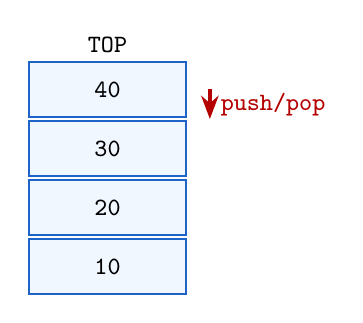
\begin{tikzpicture}[
  cell/.style={draw=pyblue, fill=pylightblue!40, minimum width=2cm, minimum height=0.7cm, thick},
  every node/.style={font=\ttfamily\small}
]
  \foreach \val/\i in {10/0, 20/1, 30/2, 40/3} {
    \node[cell] at (0, \i * 0.75) {\val};
  }
  \draw[-Stealth, very thick, pyred] (1.3, 3*0.75) -- node[right] {push/pop} (1.3, 2.5*0.75);
  \node[above=0.2cm] at (0, 3.2*0.75) {\textbf{TOP}};
\end{tikzpicture}
\caption{Stack (LIFO)}
\end{subfigure}
\hfill
\begin{subfigure}[b]{0.45\textwidth}
\centering
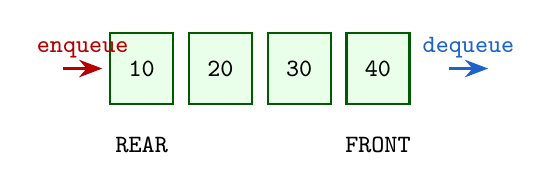
\begin{tikzpicture}[
  cell/.style={draw=pygreen!70!black, fill=pylightgreen!60, minimum width=0.8cm, minimum height=0.9cm, thick},
  every node/.style={font=\ttfamily\small}
]
  \foreach \val/\i in {10/0, 20/1, 30/2, 40/3} {
    \node[cell] at (\i * 1.0, 0) {\val};
  }
  \draw[-Stealth, very thick, pyred] (-1, 0) -- node[above] {enqueue} (-0.5, 0);
  \draw[-Stealth, very thick, pyblue] (3.5+0.4, 0) -- node[above] {dequeue} (4.4, 0);
  \node[below=0.3cm] at (0, -0.45) {\textbf{REAR}};
  \node[below=0.3cm] at (3, -0.45) {\textbf{FRONT}};
\end{tikzpicture}
\caption{Queue (FIFO)}
\end{subfigure}
\caption{Stack vs Queue operations.}
\label{fig:stack-queue}
\end{figure}

\subsection{Hash Tables}

A hash table maps keys to values using a hash function
$h: \mathcal{U} \to \{0, 1, \ldots, m-1\}$.

\begin{definition}[Load Factor]
The \emph{load factor} of a hash table with $n$ stored items and $m$ buckets is
$\alpha = n/m$.  Python's \texttt{dict} resizes when $\alpha > 2/3$.
\end{definition}

\begin{figure}[h]
\centering
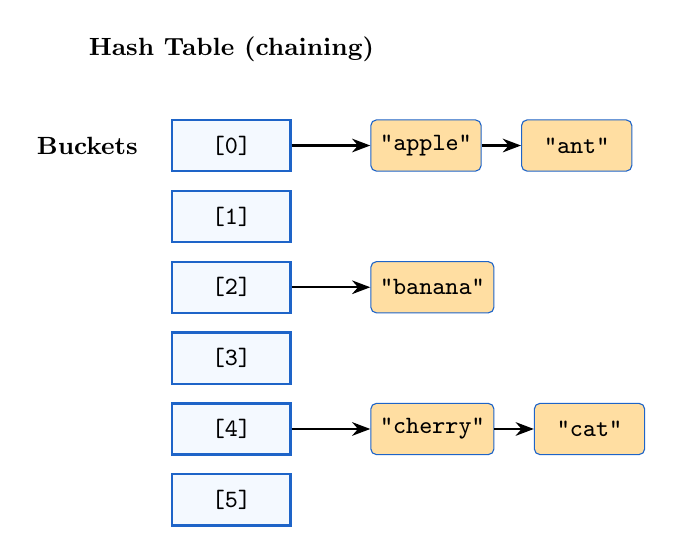
\begin{tikzpicture}[
  bucket/.style={draw=pyblue, fill=pylightblue!30, minimum width=1.5cm, minimum height=0.65cm, thick, font=\ttfamily\small},
  chain/.style={draw=pyblue, fill=nodeorange!60, minimum width=1.4cm, minimum height=0.65cm, rounded corners=2pt, font=\ttfamily\small},
  ptr/.style={-Stealth, thick}
]
  % buckets
  \foreach \i in {0,...,5} {
    \node[bucket] (b\i) at (0, -\i * 0.9) {[\i]};
  }
  % chained entries
  \node[chain, right=1cm of b0] (c00) {"apple"};
  \node[chain, right=0.5cm of c00] (c01) {"ant"};
  \draw[ptr] (b0) -- (c00);
  \draw[ptr] (c00) -- (c01);

  \node[chain, right=1cm of b2] (c20) {"banana"};
  \draw[ptr] (b2) -- (c20);

  \node[chain, right=1cm of b4] (c40) {"cherry"};
  \node[chain, right=0.5cm of c40] (c41) {"cat"};
  \draw[ptr] (b4) -- (c40);
  \draw[ptr] (c40) -- (c41);

  \node[left=0.3cm of b0, font=\bfseries\small] {Buckets};
  \node[above=0.6cm of b0, font=\bfseries\small] {Hash Table (chaining)};
\end{tikzpicture}
\caption{Hash table with separate chaining collision resolution.}
\label{fig:hash-table}
\end{figure}

% ============================================================
\section{Trees}
% ============================================================

\subsection{Binary Search Tree}

\begin{definition}[BST Property]
For every node $v$ in a binary search tree, all keys in $v$'s left subtree are
strictly less than $v$'s key, and all keys in $v$'s right subtree are strictly
greater~\cite{cormen2022}.
\end{definition}

\begin{figure}[h]
\centering
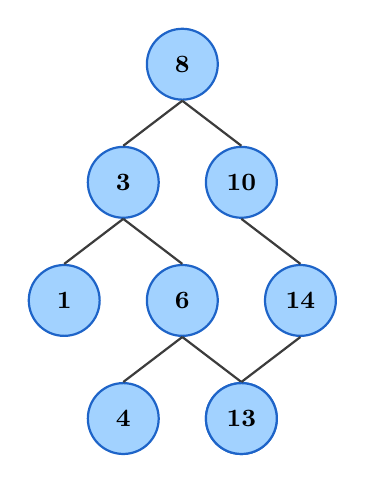
\begin{tikzpicture}[
  treenode/.style={circle, draw=pyblue, fill=nodeblue!60, thick, minimum size=0.9cm, font=\bfseries\small},
  edge from parent/.style={draw=pygray, thick}
]
  \node[treenode] (root) {8}
    child {
      node[treenode] {3}
        child { node[treenode] {1} }
        child {
          node[treenode] {6}
            child { node[treenode] {4} }
            child { node[treenode] {7} }
        }
    }
    child {
      node[treenode] {10}
        child [missing] {}
        child { node[treenode] {14}
          child { node[treenode] {13} }
          child [missing] {}
        }
    };
\end{tikzpicture}
\caption{Example Binary Search Tree (BST). In-order traversal: 1, 3, 4, 6, 7, 8, 10, 13, 14.}
\label{fig:bst}
\end{figure}

\subsection{AVL Tree Rotations}

The AVL tree~\cite{cormen2022} maintains balance using four rotation cases
(Figure~\ref{fig:avl-rotations}).

\begin{figure}[h]
\centering
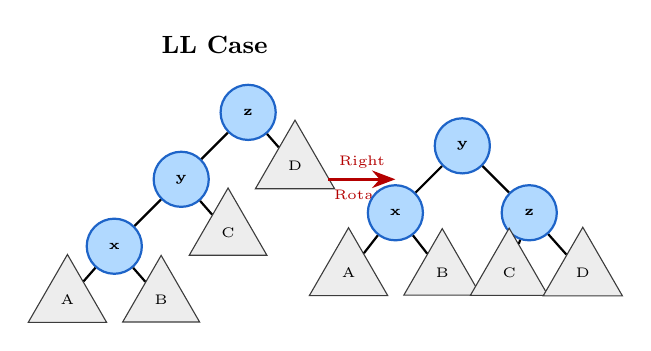
\begin{tikzpicture}[
  n/.style={circle, draw=pyblue, fill=nodeblue!50, thick, minimum size=0.7cm, font=\bfseries\tiny},
  tri/.style={regular polygon, regular polygon sides=3, draw=pygray, fill=nodegray!50, minimum size=0.6cm, font=\tiny},
  arr/.style={-Stealth, very thick, pyred},
  scale=0.85
]
  % --- Left-Left case ---
  \begin{scope}[xshift=0cm]
    \node[font=\small\bfseries] at (1.5, 2.5) {LL Case};
    % before
    \node[n] (z) at (2, 1.5) {z};
    \node[n] (y) at (1, 0.5) {y};
    \node[n] (x) at (0, -0.5) {x};
    \node[tri] (A) at (-0.7, -1.3) {A};
    \node[tri] (B) at (0.7, -1.3) {B};
    \node[tri] (C) at (1.7, -0.3) {C};
    \node[tri] (D) at (2.7, 0.7) {D};
    \draw[thick] (z)--(y)--(x); \draw[thick] (x)--(A); \draw[thick] (x)--(B);
    \draw[thick] (y)--(C); \draw[thick] (z)--(D);
    % arrow
    \draw[arr] (3.2, 0.5) -- node[above,font=\tiny] {Right} node[below,font=\tiny] {Rotate} (4.2, 0.5);
    % after
    \node[n] (y2) at (5.2, 1.0) {y};
    \node[n] (x2) at (4.2, 0.0) {x};
    \node[n] (z2) at (6.2, 0.0) {z};
    \node[tri] (A2) at (3.5, -0.9) {A};
    \node[tri] (B2) at (4.9, -0.9) {B};
    \node[tri] (C2) at (5.9, -0.9) {C};
    \node[tri] (D2) at (7.0, -0.9) {D};
    \draw[thick] (y2)--(x2)--(A2); \draw[thick] (x2)--(B2);
    \draw[thick] (y2)--(z2)--(C2); \draw[thick] (z2)--(D2);
  \end{scope}
\end{tikzpicture}
\caption{AVL Left-Left (LL) rotation: a single right rotation restores balance.}
\label{fig:avl-rotations}
\end{figure}

\subsection{Heap}

A \emph{binary min-heap} satisfies: for every node $i$, $A[i] \leq A[\text{left}(i)]$
and $A[i] \leq A[\text{right}(i)]$~\cite{cormen2022}.

\begin{figure}[h]
\centering
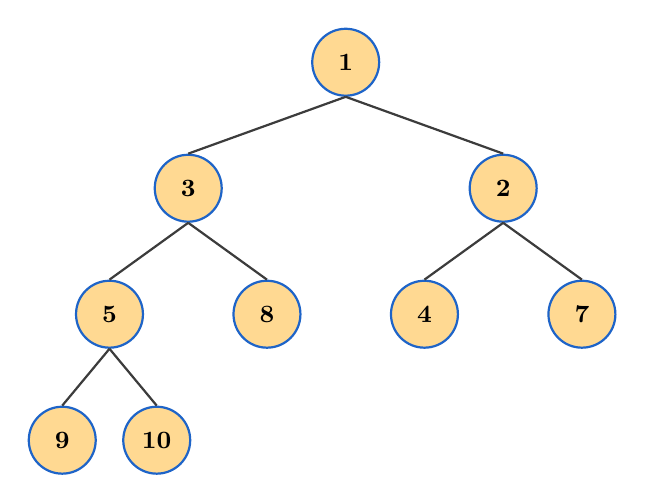
\begin{tikzpicture}[
  n/.style={circle, draw=pyblue, fill=nodeorange!70, thick, minimum size=0.85cm, font=\bfseries\small},
  edge from parent/.style={draw=pygray, thick},
  level 1/.style={sibling distance=4cm, level distance=1.6cm},
  level 2/.style={sibling distance=2cm, level distance=1.6cm},
  level 3/.style={sibling distance=1.2cm, level distance=1.6cm}
]
  \node[n] {1}
    child { node[n] {3}
      child { node[n] {5}
        child { node[n] {9} }
        child { node[n] {10} }
      }
      child { node[n] {8} }
    }
    child { node[n] {2}
      child { node[n] {4} }
      child { node[n] {7} }
    };
\end{tikzpicture}
\caption{Binary min-heap stored as an array: [1, 3, 2, 5, 8, 4, 7, 9, 10].}
\label{fig:heap}
\end{figure}

\subsection{Trie (Prefix Tree)}

\begin{figure}[h]
\centering
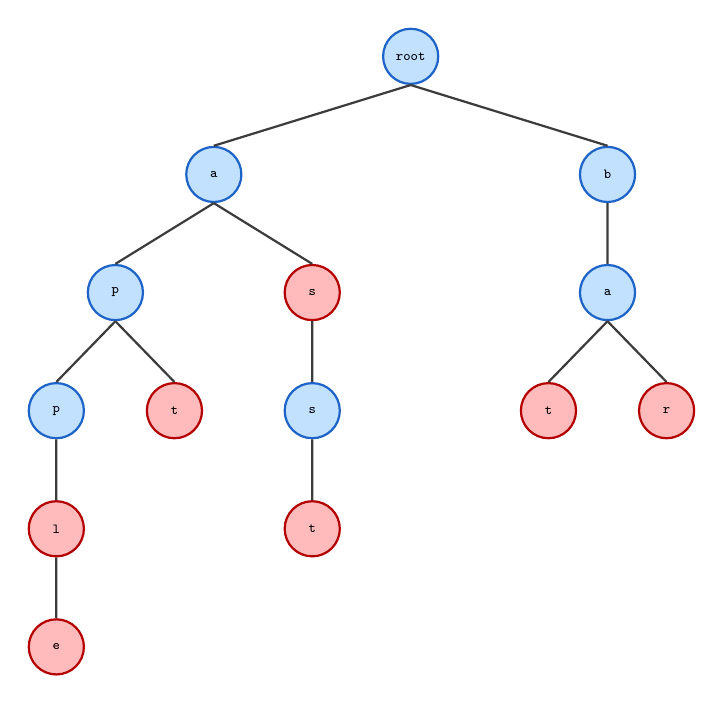
\begin{tikzpicture}[
  every node/.style={circle, draw=pyblue, fill=nodeblue!40, thick, minimum size=0.7cm, font=\ttfamily\tiny},
  endnode/.style={circle, draw=pyred, fill=nodered!50, thick, minimum size=0.7cm, font=\ttfamily\tiny},
  edge from parent/.style={draw=pygray, thick},
  level 1/.style={sibling distance=5cm, level distance=1.5cm},
  level 2/.style={sibling distance=2.5cm, level distance=1.5cm},
  level 3/.style={sibling distance=1.5cm, level distance=1.5cm}
]
  \node {root}
    child { node {a}
      child { node {p}
        child { node {p}
          child { node[endnode] {l}
            child { node[endnode] {e} }
          }
        }
        child { node[endnode] {t} }
      }
      child { node[endnode] {s}
        child { node {s}
          child { node[endnode] {t} }
        }
      }
    }
    child { node {b}
      child { node {a}
        child { node[endnode] {t} }
        child { node[endnode] {r} }
      }
    };
\end{tikzpicture}
\caption{Trie storing \textit{apple}, \textit{apt}, \textit{as}, \textit{asset},
\textit{bat}, \textit{bar}. Red nodes mark end-of-word.}
\label{fig:trie}
\end{figure}

\subsection{Segment Tree}

A segment tree for range-sum queries on array $A[0..n-1]$
stores partial sums in an implicit binary tree.

\begin{figure}[h]
\centering
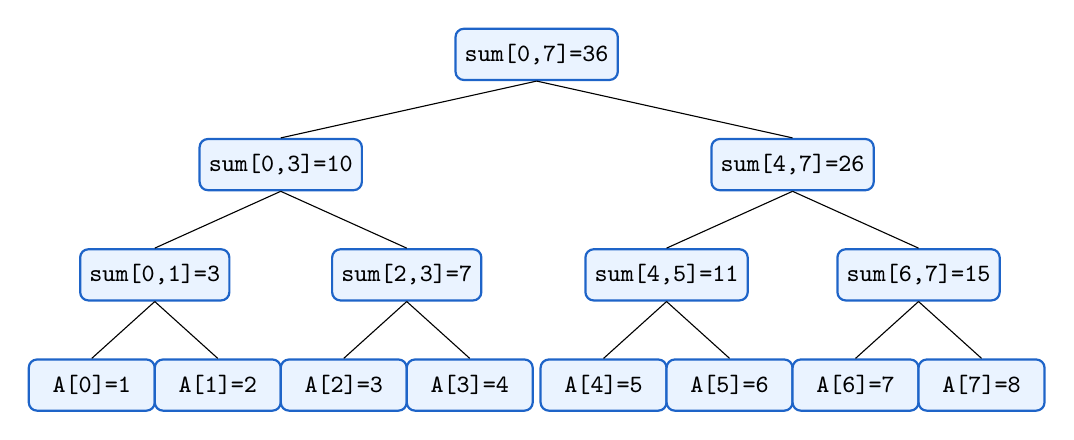
\begin{tikzpicture}[
  n/.style={rectangle, draw=pyblue, fill=pylightblue!60, thick, rounded corners=3pt,
            minimum width=1.6cm, minimum height=0.65cm, font=\ttfamily\small},
  arr/.style={-Stealth, thick, pyblue},
  level 1/.style={sibling distance=6.5cm, level distance=1.4cm},
  level 2/.style={sibling distance=3.2cm, level distance=1.4cm},
  level 3/.style={sibling distance=1.6cm, level distance=1.4cm}
]
  \node[n] {sum[0,7]=36}
    child { node[n] {sum[0,3]=10}
      child { node[n] {sum[0,1]=3}
        child { node[n] {A[0]=1} }
        child { node[n] {A[1]=2} }
      }
      child { node[n] {sum[2,3]=7}
        child { node[n] {A[2]=3} }
        child { node[n] {A[3]=4} }
      }
    }
    child { node[n] {sum[4,7]=26}
      child { node[n] {sum[4,5]=11}
        child { node[n] {A[4]=5} }
        child { node[n] {A[5]=6} }
      }
      child { node[n] {sum[6,7]=15}
        child { node[n] {A[6]=7} }
        child { node[n] {A[7]=8} }
      }
    };
\end{tikzpicture}
\caption{Segment tree for $A=[1,2,3,4,5,6,7,8]$ supporting $O(\log n)$
range-sum queries and point updates.}
\label{fig:segment-tree}
\end{figure}

\subsection{B-Tree}

B-Trees are used in databases and file systems to minimise disk I/O
by keeping many keys per node~\cite{cormen2022}.

\begin{figure}[h]
\centering
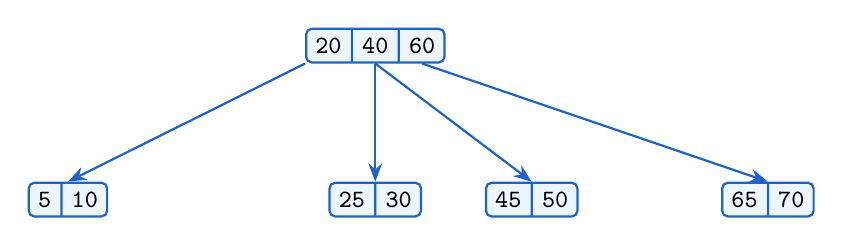
\begin{tikzpicture}[
  bnode/.style={
    rectangle split, rectangle split horizontal,
    draw=pyblue, fill=pylightblue!50, thick, rounded corners=2pt,
    font=\ttfamily\small, rectangle split part fill={pylightblue!50}
  },
  ptr/.style={-Stealth, thick, pyblue}
]
  % root
  \node[bnode, rectangle split parts=3] (root)
    {\textbf{20} \nodepart{two} \textbf{40} \nodepart{three} \textbf{60}};

  % level 1
  \node[bnode, rectangle split parts=2, below left=1.5cm and 2.5cm of root] (l1)
    {\textbf{5} \nodepart{two} \textbf{10}};
  \node[bnode, rectangle split parts=2, below=1.5cm of root] (l2)
    {\textbf{25} \nodepart{two} \textbf{30}};
  \node[bnode, rectangle split parts=2, below right=1.5cm and 0.5cm of root] (l3)
    {\textbf{45} \nodepart{two} \textbf{50}};
  \node[bnode, rectangle split parts=2, below right=1.5cm and 3.5cm of root] (l4)
    {\textbf{65} \nodepart{two} \textbf{70}};

  \draw[ptr] (root.south west) -- (l1.north);
  \draw[ptr] (root.south)      -- (l2.north);
  \draw[ptr] (root.two south)  -- (l3.north);
  \draw[ptr] (root.three south) -- (l4.north);
\end{tikzpicture}
\caption{B-Tree of minimum degree $t=2$ (order 4). Each internal node holds 1–3 keys.}
\label{fig:btree}
\end{figure}

% ============================================================
\section{Graphs}
% ============================================================

\subsection{Representations}

\begin{figure}[h]
\centering
\begin{subfigure}[b]{0.30\textwidth}
\centering
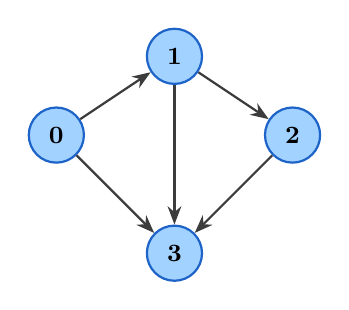
\begin{tikzpicture}[
  v/.style={circle, draw=pyblue, fill=nodeblue!60, thick, minimum size=0.7cm, font=\bfseries\small},
  e/.style={-Stealth, thick, pygray}
]
  \node[v] (0) at (0,1.5) {0};
  \node[v] (1) at (1.5,2.5) {1};
  \node[v] (2) at (3,1.5) {2};
  \node[v] (3) at (1.5,0) {3};
  \draw[e] (0)--(1); \draw[e] (0)--(3);
  \draw[e] (1)--(2); \draw[e] (2)--(3);
  \draw[e] (1)--(3);
\end{tikzpicture}
\caption{Graph}
\end{subfigure}
\hfill
\begin{subfigure}[b]{0.32\textwidth}
\centering
$\begin{pmatrix}
0 & 1 & 0 & 1 \\
1 & 0 & 1 & 1 \\
0 & 1 & 0 & 1 \\
1 & 1 & 1 & 0
\end{pmatrix}$
\caption{Adjacency Matrix}
\end{subfigure}
\hfill
\begin{subfigure}[b]{0.32\textwidth}
\centering
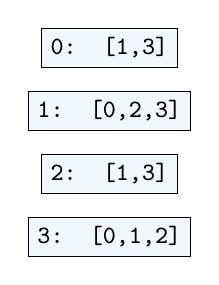
\begin{tikzpicture}[font=\ttfamily\small]
  \node[draw, fill=pylightblue!40] (r0) at (0,3) {0: [1,3]};
  \node[draw, fill=pylightblue!40] (r1) at (0,2.2) {1: [0,2,3]};
  \node[draw, fill=pylightblue!40] (r2) at (0,1.4) {2: [1,3]};
  \node[draw, fill=pylightblue!40] (r3) at (0,0.6) {3: [0,1,2]};
\end{tikzpicture}
\caption{Adjacency List}
\end{subfigure}
\caption{Three representations of the same undirected graph.}
\label{fig:graph-repr}
\end{figure}

\subsection{BFS and DFS}

\begin{algorithm}
\caption{Breadth-First Search (BFS)~\cite{cormen2022}}
\begin{algorithmic}[1]
\Procedure{BFS}{$G, s$}
  \State Initialise distance $d[v] \leftarrow \infty$ for all $v$; $d[s] \leftarrow 0$
  \State Enqueue $s$ into $Q$
  \While{$Q \neq \emptyset$}
    \State $u \leftarrow$ Dequeue($Q$)
    \For{each neighbour $v$ of $u$}
      \If{$d[v] = \infty$}
        \State $d[v] \leftarrow d[u] + 1$
        \State Enqueue $v$ into $Q$
      \EndIf
    \EndFor
  \EndWhile
\EndProcedure
\end{algorithmic}
\end{algorithm}

\subsection{Dijkstra's Algorithm}

\begin{theorem}[Dijkstra Correctness~\cite{dijkstra1959,cormen2022}]
When all edge weights are non-negative, Dijkstra's algorithm correctly
computes shortest-path distances from a source $s$ to all reachable vertices.
The time complexity with a binary heap is $O((V+E)\log V)$.
\end{theorem}

\begin{algorithm}
\caption{Dijkstra's Shortest Path~\cite{dijkstra1959}}
\begin{algorithmic}[1]
\Procedure{Dijkstra}{$G, w, s$}
  \For{each vertex $v \in V$}
    \State $d[v] \leftarrow \infty$; $\pi[v] \leftarrow \textsc{nil}$
  \EndFor
  \State $d[s] \leftarrow 0$
  \State $Q \leftarrow$ MinPriorityQueue($V$, key $= d$)
  \While{$Q \neq \emptyset$}
    \State $u \leftarrow$ ExtractMin($Q$)
    \For{each $(u,v) \in E$}
      \If{$d[u] + w(u,v) < d[v]$}
        \State $d[v] \leftarrow d[u] + w(u,v)$
        \State $\pi[v] \leftarrow u$
        \State DecreaseKey($Q$, $v$, $d[v]$)
      \EndIf
    \EndFor
  \EndWhile
\EndProcedure
\end{algorithmic}
\end{algorithm}

% ============================================================
\section{Advanced and Modern Data Structures}
% ============================================================

\subsection{Bloom Filter}

A Bloom filter~\cite{bloom1970} uses $k$ independent hash functions and a bit array
of size $m$ to achieve membership queries with \emph{no false negatives} and
a bounded false-positive probability.

\begin{theorem}[Bloom Filter False-Positive Rate~\cite{bloom1970}]
For a Bloom filter with $m$ bits and $k$ hash functions storing $n$ elements,
the false-positive probability is approximately:
\[
  \varepsilon \approx \left(1 - e^{-kn/m}\right)^k
\]
The optimal number of hash functions is $k^* = \frac{m}{n}\ln 2$.
\end{theorem}

\begin{figure}[h]
\centering
\begin{tikzpicture}[font=\ttfamily\small, scale=0.9]
  % bit array
  \foreach \i/\v in {0/0,1/1,2/0,3/1,4/0,5/1,6/0,7/1,8/0,9/1} {
    \draw[draw=pyblue, fill={ifodd\i pylightblue!80 \else white \fi}]
      (\i*0.9, 0) rectangle (\i*0.9+0.85, 0.75)
      node[midway] {\v};
  }
  % label
  \node[left=0.2cm, font=\small\bfseries] at (0, 0.375) {Bits:};

  % hash arrows for item "cat"
  \node[draw=pyred, rounded corners, fill=nodered!30, font=\small] (item) at (3.8, 2.0) {"cat"};
  \draw[-Stealth, thick, pyred!80] (item) -- node[left, font=\tiny] {$h_1$} (0.9*1+0.4, 0.75);
  \draw[-Stealth, thick, pyred!80] (item) -- node[right, font=\tiny] {$h_2$} (0.9*5+0.4, 0.75);
  \draw[-Stealth, thick, pyred!80] (item) -- node[right, font=\tiny] {$h_3$} (0.9*7+0.4, 0.75);

  \node[below=0.4cm] at (4.0, 0) {Bloom Filter Bit Array ($m=10$)};
\end{tikzpicture}
\caption{Bloom filter: inserting \texttt{"cat"} sets bits at positions
$h_1(\text{"cat"})=1$, $h_2(\text{"cat"})=5$, $h_3(\text{"cat"})=7$.}
\label{fig:bloom-filter}
\end{figure}

\subsection{Skip List}

A skip list~\cite{pugh1990} is a randomised data structure with $O(\log n)$
expected time for search, insert and delete.

\begin{figure}[h]
\centering
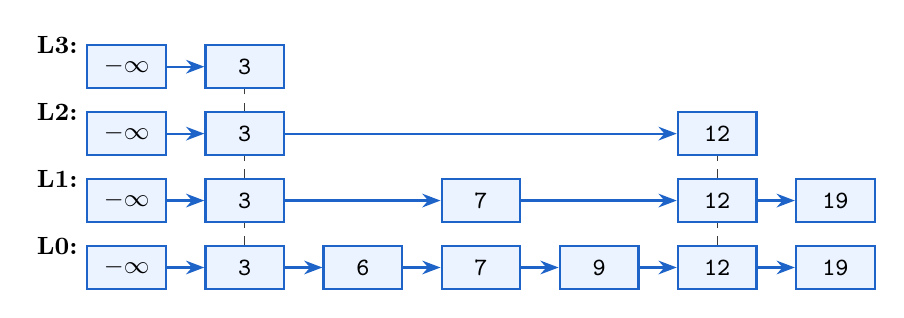
\begin{tikzpicture}[
  sn/.style={draw=pyblue, fill=pylightblue!60, minimum width=1.0cm, minimum height=0.55cm, thick, font=\ttfamily\small},
  ptr/.style={-Stealth, thick, pyblue},
  lbl/.style={font=\small\bfseries, left}
]
  % levels
  \foreach \level/\y in {0/0, 1/0.85, 2/1.7, 3/2.55} {
    \node[lbl] at (-0.5, \y+0.27) {L\level:};
  }

  % sentinels
  \node[sn] (hd0) at (0,0)    {$-\infty$};
  \node[sn] (hd1) at (0,0.85) {$-\infty$};
  \node[sn] (hd2) at (0,1.7)  {$-\infty$};
  \node[sn] (hd3) at (0,2.55) {$-\infty$};

  % nodes at level 0 (all)
  \foreach \v/\x in {3/1.5, 6/3.0, 7/4.5, 9/6.0, 12/7.5, 19/9.0} {
    \node[sn] (n0\v) at (\x, 0) {\v};
  }
  % nodes at level 1
  \foreach \v/\x in {3/1.5, 7/4.5, 12/7.5, 19/9.0} {
    \node[sn] (n1\v) at (\x, 0.85) {\v};
  }
  % nodes at level 2
  \foreach \v/\x in {3/1.5, 12/7.5} {
    \node[sn] (n2\v) at (\x, 1.7) {\v};
  }
  % node at level 3
  \node[sn] (n33) at (1.5, 2.55) {3};

  % horizontal pointers level 0
  \draw[ptr] (hd0) -- (n03);
  \foreach \a/\b in {3/6,6/7,7/9,9/12,12/19} { \draw[ptr] (n0\a) -- (n0\b); }

  % level 1
  \draw[ptr] (hd1) -- (n13);
  \foreach \a/\b in {3/7,7/12,12/19} { \draw[ptr] (n1\a) -- (n1\b); }

  % level 2
  \draw[ptr] (hd2) -- (n23);
  \draw[ptr] (n23) -- (n212);

  % level 3
  \draw[ptr] (hd3) -- (n33);

  % vertical links for node 3
  \draw[dashed, pygray] (n03) -- (n13) -- (n23) -- (n33);
  % vertical links for node 12
  \draw[dashed, pygray] (n012) -- (n112) -- (n212);
\end{tikzpicture}
\caption{Skip list with four levels storing $\{3,6,7,9,12,19\}$.
Search for 9 traverses: L3$\to$L2$\to$L1$\to$L0 in $O(\log n)$ expected.}
\label{fig:skip-list}
\end{figure}

\subsection{Disjoint Set Union (Union-Find)}

\begin{theorem}[Inverse Ackermann~\cite{tarjan1975}]
With \emph{path compression} and \emph{union by rank}, a sequence of $m$
Union/Find operations on $n$ elements runs in $O(m\,\alpha(n))$ time,
where $\alpha$ is the inverse Ackermann function — effectively constant for
all practical inputs.
\end{theorem}

\subsection{Van Emde Boas Tree}

\begin{theorem}[vEB Complexity~\cite{vanembdeboas1977}]
A van Emde Boas tree on universe $\{0,\ldots,U-1\}$ supports
Insert, Delete, Successor, Predecessor, Minimum, and Maximum
in $O(\log\log U)$ worst-case time and uses $O(U)$ space.
\end{theorem}

% ============================================================
\section{Algorithms}
% ============================================================

\subsection{Sorting}

\begin{table}[h]
\centering
\caption{Comparison of sorting algorithms~\cite{cormen2022,sedgewick2011}.}
\begin{tabular}{lccccl}
\toprule
\textbf{Algorithm} & \textbf{Best} & \textbf{Average} & \textbf{Worst} & \textbf{Space} & \textbf{Stable} \\
\midrule
Bubble Sort     & $O(n)$      & $O(n^2)$      & $O(n^2)$      & $O(1)$       & Yes \\
Insertion Sort  & $O(n)$      & $O(n^2)$      & $O(n^2)$      & $O(1)$       & Yes \\
Merge Sort      & $O(n\log n)$& $O(n\log n)$  & $O(n\log n)$  & $O(n)$       & Yes \\
Quick Sort      & $O(n\log n)$& $O(n\log n)$  & $O(n^2)$      & $O(\log n)$  & No  \\
Heap Sort       & $O(n\log n)$& $O(n\log n)$  & $O(n\log n)$  & $O(1)$       & No  \\
Counting Sort   & $O(n+k)$    & $O(n+k)$      & $O(n+k)$      & $O(k)$       & Yes \\
Radix Sort      & $O(nk)$     & $O(nk)$       & $O(nk)$       & $O(n+k)$     & Yes \\
Tim Sort        & $O(n)$      & $O(n\log n)$  & $O(n\log n)$  & $O(n)$       & Yes \\
\bottomrule
\end{tabular}
\end{table}

\subsection{Growth Rate Comparison}

\begin{figure}[h]
\centering
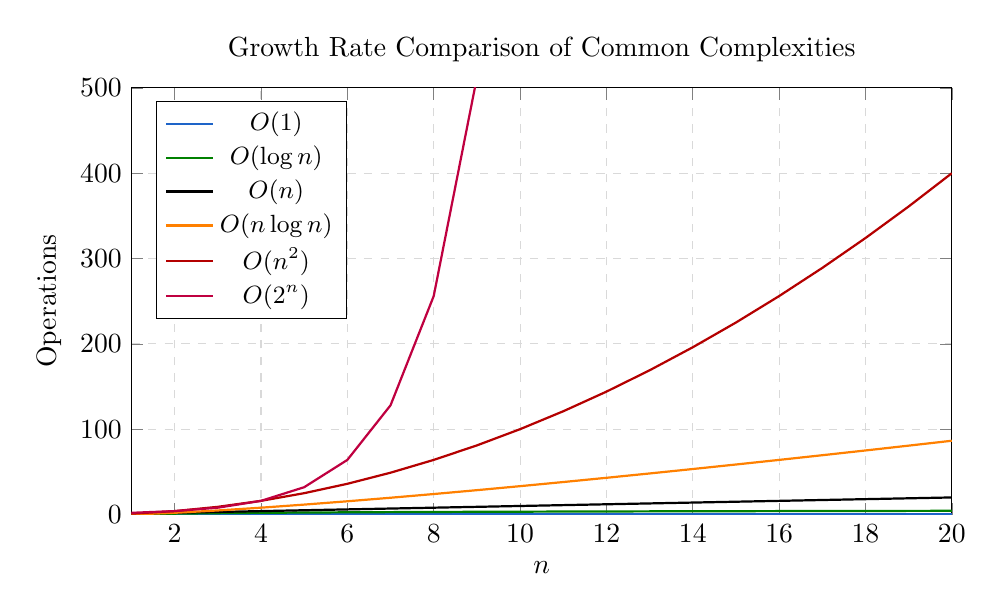
\begin{tikzpicture}
\begin{axis}[
  width=12cm, height=7cm,
  xlabel={$n$},
  ylabel={Operations},
  xmin=1, xmax=20,
  ymin=0, ymax=500,
  legend pos=north west,
  legend style={font=\small},
  grid=major,
  grid style={dashed, gray!30},
  title={Growth Rate Comparison of Common Complexities}
]
  \addplot[thick, pyblue,   domain=1:20, samples=20] {1};         \addlegendentry{$O(1)$}
  \addplot[thick, pygreen,  domain=1:20, samples=20] {ln(x)/ln(2)};\addlegendentry{$O(\log n)$}
  \addplot[thick, black,    domain=1:20, samples=20] {x};          \addlegendentry{$O(n)$}
  \addplot[thick, orange,   domain=1:20, samples=20] {x*ln(x)/ln(2)};\addlegendentry{$O(n\log n)$}
  \addplot[thick, pyred,    domain=1:20, samples=20] {x^2};        \addlegendentry{$O(n^2)$}
  \addplot[thick, purple,   domain=1:14, samples=14] {2^x};        \addlegendentry{$O(2^n)$}
\end{axis}
\end{tikzpicture}
\caption{Growth rates of common time complexities.}
\label{fig:growth}
\end{figure}

\subsection{Master Theorem}

\begin{theorem}[Master Theorem~\cite{cormen2022}]
Let $T(n) = aT(n/b) + f(n)$ where $a \geq 1$, $b > 1$, $f$ asymptotically positive.
Set $c^* = \log_b a$.
\begin{enumerate}[label=\textbf{Case \arabic*:}]
  \item If $f(n) = O(n^{c^*-\varepsilon})$ for some $\varepsilon > 0$:
        $T(n) = \Theta(n^{c^*})$.
  \item If $f(n) = \Theta(n^{c^*}\log^k n)$ for some $k \geq 0$:
        $T(n) = \Theta(n^{c^*}\log^{k+1} n)$.
  \item If $f(n) = \Omega(n^{c^*+\varepsilon})$ and regularity holds:
        $T(n) = \Theta(f(n))$.
\end{enumerate}
\end{theorem}

\subsection{Dynamic Programming — Optimal Substructure}

\begin{definition}[Optimal Substructure]
A problem has \emph{optimal substructure} if an optimal solution contains
optimal solutions to its sub-problems~\cite{cormen2022}.
\end{definition}

\begin{algorithm}
\caption{Longest Common Subsequence (LCS)}
\begin{algorithmic}[1]
\Procedure{LCS}{$X[1..m], Y[1..n]$}
  \For{$i = 0$ to $m$} $c[i][0] \leftarrow 0$ \EndFor
  \For{$j = 0$ to $n$} $c[0][j] \leftarrow 0$ \EndFor
  \For{$i = 1$ to $m$}
    \For{$j = 1$ to $n$}
      \If{$X[i] = Y[j]$}
        \State $c[i][j] \leftarrow c[i-1][j-1] + 1$
      \Else
        \State $c[i][j] \leftarrow \max(c[i-1][j],\; c[i][j-1])$
      \EndIf
    \EndFor
  \EndFor
  \Return $c[m][n]$
\EndProcedure
\end{algorithmic}
\end{algorithm}

% ============================================================
\section{Data Management and Governance}
% ============================================================

\subsection{Data Quality Dimensions}

\begin{figure}[h]
\centering
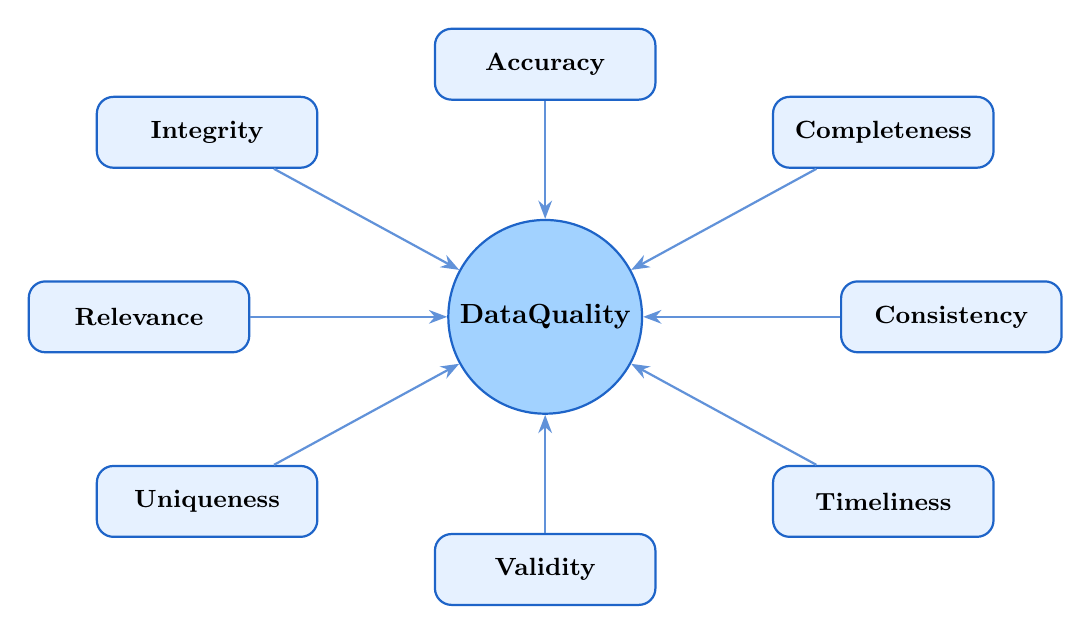
\begin{tikzpicture}[
  dim/.style={
    rectangle, rounded corners=6pt, draw=pyblue, fill=pylightblue!70, thick,
    minimum width=2.8cm, minimum height=0.9cm, font=\small\bfseries, text centered
  },
  centre/.style={
    circle, draw=pyblue, fill=nodeblue!60, thick,
    minimum size=2.2cm, font=\bfseries, text centered
  },
  arr/.style={-Stealth, thick, pyblue!70}
]
  \node[centre] (dq) {Data\\Quality};
  \node[dim, above=1.5cm of dq]       (acc) {Accuracy};
  \node[dim, above right=1.0cm and 2.0cm of dq] (comp) {Completeness};
  \node[dim, right=2.5cm of dq]       (cons) {Consistency};
  \node[dim, below right=1.0cm and 2.0cm of dq] (time) {Timeliness};
  \node[dim, below=1.5cm of dq]       (val)  {Validity};
  \node[dim, below left=1.0cm and 2.0cm of dq]  (uni)  {Uniqueness};
  \node[dim, left=2.5cm of dq]        (rel)  {Relevance};
  \node[dim, above left=1.0cm and 2.0cm of dq]  (inte) {Integrity};

  \foreach \n in {acc,comp,cons,time,val,uni,rel,inte} {
    \draw[arr] (\n) -- (dq);
  }
\end{tikzpicture}
\caption{Eight dimensions of data quality used in data governance frameworks.}
\label{fig:data-quality}
\end{figure}

\subsection{Data Pipeline Architecture}

\begin{figure}[h]
\centering
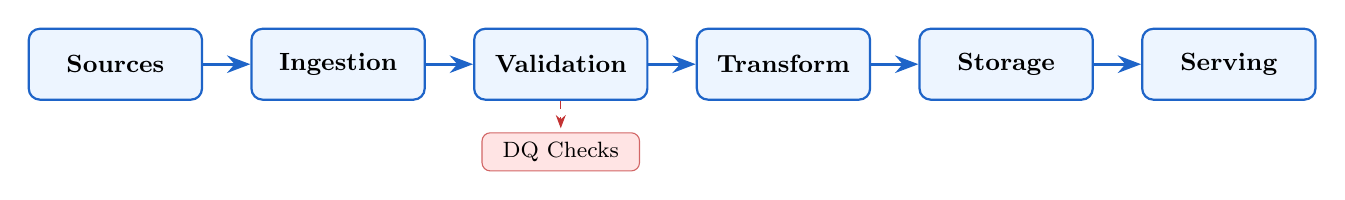
\begin{tikzpicture}[
  stage/.style={
    rectangle, draw=pyblue, fill=pylightblue!50, thick, rounded corners=4pt,
    minimum width=2.2cm, minimum height=0.9cm, font=\small\bfseries, text centered
  },
  arr/.style={-Stealth, very thick, pyblue},
  node distance=0.6cm
]
  \node[stage] (src)  {Sources};
  \node[stage, right=of src]  (ing)  {Ingestion};
  \node[stage, right=of ing]  (val)  {Validation};
  \node[stage, right=of val]  (trans){Transform};
  \node[stage, right=of trans](store){Storage};
  \node[stage, right=of store](serve){Serving};

  \draw[arr] (src)  -- (ing);
  \draw[arr] (ing)  -- (val);
  \draw[arr] (val)  -- (trans);
  \draw[arr] (trans)-- (store);
  \draw[arr] (store)-- (serve);

  \node[below=0.4cm of val, draw=pyred!60, fill=nodered!20, rounded corners=3pt,
        font=\footnotesize, minimum width=2cm] {DQ Checks};
  \draw[-Stealth, pyred!80, dashed] (val.south) -- +(0,-0.35);
\end{tikzpicture}
\caption{Generic data pipeline architecture with data quality (DQ) checks at the validation stage.}
\label{fig:pipeline}
\end{figure}

\subsection{Consistent Hashing in Distributed Systems}

\begin{figure}[h]
\centering
\begin{tikzpicture}[scale=1.0]
  % ring
  \draw[thick, pyblue] (0,0) circle(2.5cm);

  % virtual nodes
  \foreach \angle/\label/\col in {
    0/Node A/nodeblue,
    60/Node B/nodeorange,
    140/Node C/pylightgreen!80!black,
    200/Node A/nodeblue,
    280/Node B/nodeorange,
    330/Node C/pylightgreen!80!black
  } {
    \fill[\col!80] ({2.5*cos(\angle)}, {2.5*sin(\angle)}) circle(0.25cm);
    \node[font=\tiny\bfseries] at ({2.9*cos(\angle)}, {2.9*sin(\angle)}) {\label};
  }

  % keys
  \foreach \angle/\k in {20/k1, 80/k2, 170/k3, 240/k4} {
    \fill[pyred!70] ({2.5*cos(\angle)}, {2.5*sin(\angle)}) circle(0.12cm);
    \node[font=\tiny, pyred] at ({2.15*cos(\angle)}, {2.15*sin(\angle)}) {\k};
  }

  \node[font=\small\bfseries] at (0,0) {Hash Ring};
\end{tikzpicture}
\caption{Consistent hashing ring: virtual nodes from three physical nodes
($A$, $B$, $C$) are distributed around the ring.
Keys are assigned to the nearest node in clockwise order.}
\label{fig:consistent-hash}
\end{figure}

% ============================================================
\section{Python-Specific Idioms Summary}
% ============================================================

\begin{table}[h]
\centering
\caption{Python built-in data structures and their underlying implementations.}
\begin{tabular}{lll}
\toprule
\textbf{Python Type} & \textbf{Underlying Structure} & \textbf{Key Operations} \\
\midrule
\texttt{list}        & Dynamic array          & $O(1)^*$ append, $O(n)$ insert \\
\texttt{deque}       & Doubly-linked list     & $O(1)$ append/popleft \\
\texttt{dict}        & Hash table (open addr) & $O(1)^*$ get/set/del \\
\texttt{set}         & Hash table (no values) & $O(1)^*$ add/discard \\
\texttt{heapq}       & Binary min-heap        & $O(\log n)$ push/pop \\
\texttt{SortedList}  & List-of-lists          & $O(\sqrt{n})^*$ add/del \\
\texttt{lru\_cache}  & Dict + Doubly-LL       & $O(1)$ get/put \\
\bottomrule
\end{tabular}
\end{table}

% ============================================================
%  BIBLIOGRAPHY
% ============================================================
\clearpage
\printbibliography[heading=bibintoc, title={References}]

% ---- NOTE: save the block below as references.bib in the same directory ----
%
% @book{cormen2022,
%   author    = {Cormen, Thomas H. and Leiserson, Charles E. and Rivest, Ronald L. and Stein, Clifford},
%   title     = {Introduction to Algorithms},
%   edition   = {4},
%   publisher = {MIT Press},
%   year      = {2022}
% }
% @book{sedgewick2011,
%   author    = {Sedgewick, Robert and Wayne, Kevin},
%   title     = {Algorithms},
%   edition   = {4},
%   publisher = {Addison-Wesley Professional},
%   year      = {2011}
% }
% @book{knuth1997v1,
%   author    = {Knuth, Donald E.},
%   title     = {The Art of Computer Programming, Volume 1: Fundamental Algorithms},
%   edition   = {3},
%   publisher = {Addison-Wesley},
%   year      = {1997}
% }
% @book{goodrich2013,
%   author    = {Goodrich, Michael T. and Tamassia, Roberto and Goldwasser, Michael H.},
%   title     = {Data Structures and Algorithms in Python},
%   publisher = {Wiley},
%   year      = {2013}
% }
% @book{gamma1994,
%   author    = {Gamma, Erich and Helm, Richard and Johnson, Ralph and Vlissides, John},
%   title     = {Design Patterns: Elements of Reusable Object-Oriented Software},
%   publisher = {Addison-Wesley},
%   year      = {1994}
% }
% @book{skiena2020,
%   author    = {Skiena, Steven S.},
%   title     = {The Algorithm Design Manual},
%   edition   = {3},
%   publisher = {Springer},
%   year      = {2020}
% }
% @book{okasaki1998,
%   author    = {Okasaki, Chris},
%   title     = {Purely Functional Data Structures},
%   publisher = {Cambridge University Press},
%   year      = {1998}
% }
% @book{lutz2013,
%   author    = {Lutz, Mark},
%   title     = {Learning Python},
%   edition   = {5},
%   publisher = {O'Reilly Media},
%   year      = {2013}
% }
% @book{ramalho2022,
%   author    = {Ramalho, Luciano},
%   title     = {Fluent Python},
%   edition   = {2},
%   publisher = {O'Reilly Media},
%   year      = {2022}
% }
% @article{bloom1970,
%   author    = {Bloom, Burton H.},
%   title     = {Space/time trade-offs in hash coding with allowable errors},
%   journal   = {Communications of the ACM},
%   volume    = {13},
%   number    = {7},
%   pages     = {422--426},
%   year      = {1970}
% }
% @article{pugh1990,
%   author    = {Pugh, William},
%   title     = {Skip lists: a probabilistic alternative to balanced trees},
%   journal   = {Communications of the ACM},
%   volume    = {33},
%   number    = {6},
%   pages     = {668--676},
%   year      = {1990}
% }
% @article{dijkstra1959,
%   author    = {Dijkstra, Edsger W.},
%   title     = {A note on two problems in connexion with graphs},
%   journal   = {Numerische Mathematik},
%   volume    = {1},
%   number    = {1},
%   pages     = {269--271},
%   year      = {1959}
% }
% @article{bellman1958,
%   author    = {Bellman, Richard},
%   title     = {On a routing problem},
%   journal   = {Quarterly of Applied Mathematics},
%   volume    = {16},
%   number    = {1},
%   pages     = {87--90},
%   year      = {1958}
% }
% @article{floyd1962,
%   author    = {Floyd, Robert W.},
%   title     = {Algorithm 97: Shortest path},
%   journal   = {Communications of the ACM},
%   volume    = {5},
%   number    = {6},
%   pages     = {345},
%   year      = {1962}
% }
% @article{kruskal1956,
%   author    = {Kruskal, Joseph B.},
%   title     = {On the shortest spanning subtree of a graph and the traveling salesman problem},
%   journal   = {Proceedings of the American Mathematical Society},
%   volume    = {7},
%   number    = {1},
%   pages     = {48--50},
%   year      = {1956}
% }
% @article{tarjan1975,
%   author    = {Tarjan, Robert E.},
%   title     = {Efficiency of a good but not linear set union algorithm},
%   journal   = {Journal of the ACM},
%   volume    = {22},
%   number    = {2},
%   pages     = {215--225},
%   year      = {1975}
% }
% @article{knuth1977kmp,
%   author    = {Knuth, Donald E. and Morris, James H. and Pratt, Vaughan R.},
%   title     = {Fast pattern matching in strings},
%   journal   = {SIAM Journal on Computing},
%   volume    = {6},
%   number    = {2},
%   pages     = {323--350},
%   year      = {1977}
% }
% @article{karp1987,
%   author    = {Karp, Richard M. and Rabin, Michael O.},
%   title     = {Efficient randomized pattern-matching algorithms},
%   journal   = {IBM Journal of Research and Development},
%   volume    = {31},
%   number    = {2},
%   pages     = {249--260},
%   year      = {1987}
% }
% @article{fredman1987,
%   author    = {Fredman, Michael L. and Tarjan, Robert E.},
%   title     = {Fibonacci heaps and their uses in improved network optimization algorithms},
%   journal   = {Journal of the ACM},
%   volume    = {34},
%   number    = {3},
%   pages     = {596--615},
%   year      = {1987}
% }
% @article{vanembdeboas1977,
%   author    = {van Emde Boas, Peter},
%   title     = {Preserving order in a forest in less than logarithmic time and linear space},
%   journal   = {Information Processing Letters},
%   volume    = {6},
%   number    = {3},
%   pages     = {80--82},
%   year      = {1977}
% }
% @inproceedings{kasai2001,
%   author    = {Kasai, Toru and Lee, Gunho and Arimura, Hiroki and Arikawa, Setsuo and Park, Kunsoo},
%   title     = {Linear-time longest-common-prefix computation in suffix arrays and its applications},
%   booktitle = {Combinatorial Pattern Matching (CPM 2001)},
%   series    = {Lecture Notes in Computer Science},
%   volume    = {2089},
%   pages     = {181--192},
%   publisher = {Springer},
%   year      = {2001}
% }
% @article{aho1975,
%   author    = {Aho, Alfred V. and Corasick, Margaret J.},
%   title     = {Efficient string matching: An aid to bibliographic search},
%   journal   = {Communications of the ACM},
%   volume    = {18},
%   number    = {6},
%   pages     = {333--340},
%   year      = {1975}
% }

\end{document}
